\begin{wrapfigure}[0]{r}[0cm]{10cm}
 \vspace{-7cm}
  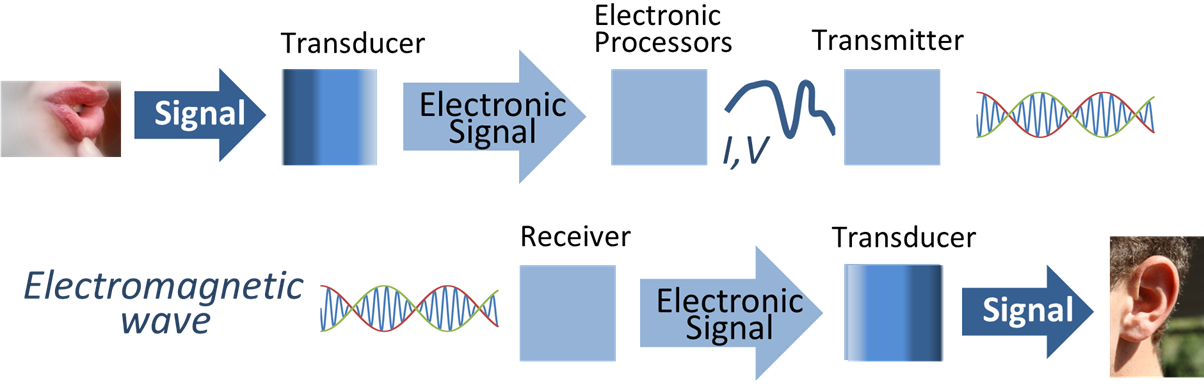
\includegraphics[scale=0.35]{Senden/Bilder/Signal_processing_system.png}
 \vspace{-7cm}
\end{wrapfigure}

\section*{Theorie- und Prüfungsfragen}


\subsection*{Oszillator}

\begin{enumerate} 
	\item[1] \emph{\textbf{TG101}} Was verstehen Sie unter einem Oszillator?
	\begin{enumerate}
	\itemsep1pt\parskip0pt\parsep0pt
		\item[A] Es ist ein sehr schmales Filter.
		\item[B] Es ist ein Messgerät zur Anzeige von Schwingungen.
		\item[C] Es ist ein FM-Modulator.
		\item[D] Es ist ein Schwingungserzeuger.
		\loesung{Lösung D}
	\end{enumerate} 
	\item[2] \emph{\textbf{TD602}}  Was ist ein LC-Oszillator? Es ist ein Schwingungs-erzeuger, wobei die Frequenz ...
	\begin{enumerate}
	\itemsep1pt\parskip0pt\parsep0pt
		\item[A] durch einen hochstabilen Quarz bestimmt wird.
		\item[B] mittels LC-Tiefpass gefiltert wird.
		\item[C] von einer Spule und einem Kondensator (LC-Schwingkreis) bestimmt wird.
		\item[D] mittels LC-Hochpass gefiltert wird.
		\loesung{Lösung C}
	\end{enumerate} 
	\item[3] \emph{\textbf{TD604}}  Wie verhält sich die Frequenz eines LC-Oszillators bei Temperaturanstieg, wenn die Kapazität des Schwingkreiskondensators mit dem Temperaturanstieg geringer wird?
	\begin{enumerate}
	\itemsep1pt\parskip0pt\parsep0pt
		\item[A] Die Schwingungen reißen ab (Aussetzer).
		\item[B] Die Frequenz wird erhöht.
		\item[C] Die Frequenz wird niedriger.
		\item[D] Die Frequenz bleibt stabil.
		\loesung{Lösung B}
	\end{enumerate} 
\end{enumerate}

\subsection*{Mischung}

\begin{enumerate} 
	\item[4] \emph{\textbf{TG102}} Welche der nachfolgenden Antworten trifft für die Wirkungsweise eines Transverters zu?
	\begin{enumerate}
	\itemsep1pt\parskip0pt\parsep0pt
		\item[A] Ein Transverter setzt beim Senden als auch beim Empfangen z.B. ein 70-cm-Signal in das 10-m-Band um.
		\item[B] Ein Transverter setzt beim Senden als auch beim Empfangen z.B. ein frequenzmoduliertes Signal in ein amplitudenmoduliertes Signal um.
		\item[C] Ein Transverter setzt beim Empfangen z.B. ein 70-cm-Signal in das 10-m-Band und beim Senden das 10-m-Sendesignal auf das 70-cm-Band um.
		\item[D] Ein Transverter setzt nur den zu empfangenden Frequenzbereich in einen anderen Frequenzbereich um, z.B. das 70-cm-Band in das 10-m-Band.
		\loesung{Lösung C}
	\end{enumerate} 
	\item[5] \emph{\textbf{TF107 }} Einem Mischer werden die Frequenzen 28 MHz und 38,7 MHz zugeführt. Welche Frequenzen werden beim Mischvorgang erzeugt?
	\begin{enumerate}
	\itemsep1pt\parskip0pt\parsep0pt
		\item[A] 10,7 MHz und 56 MHz
		\item[B] 10,7 MHz
		\item[C]  56 MHz und 66,7 MHz
		\item[D] 10,7 MHz und 66,7 MHz
		\loesung{Lösung D}
	\end{enumerate} 
	\item[6] \emph{\textbf{TF109}} Die Frequenzdifferenz zwischen dem HF-Nutzsignal und dem Spiegelsignal entspricht ...
	\begin{enumerate}
	\itemsep1pt\parskip0pt\parsep0pt
		\item[A] dem zweifachen der ersten ZF. 
		\item[B] der Frequenz des lokalen Oszillators.
		\item[C] der HF-Eingangsfrequenz.
		\item[D] der Frequenz des Preselektors.
		\loesung{Lösung A}
	\end{enumerate} 
	\item[7] \emph{\textbf{TF104}} Ein Empfänger hat eine ZF von 10,7 MHz und ist auf 28,5 MHz abgestimmt. Der Oszillator des Empfängers schwingt oberhalb der Empfangsfrequenz. Welche Frequenz hat die Spiegelfrequenz?
	\begin{enumerate}
	\itemsep1pt\parskip0pt\parsep0pt
		\item[A] 17,8 MHz 
		\item[B] 39,2 MHz
		\item[C] 48,9 MHz 
		\item[D] 49,9 MHz
		\loesung{Lösung D; $f_{sp}=f_e + 2 \cdot f_z$}
	\end{enumerate} 
	\item[8] \emph{\textbf{TF101}} Eine hohe erste ZF vereinfacht die Filterung zur Vermeidung von ...
	\begin{enumerate}
	\itemsep1pt\parskip0pt\parsep0pt
		\item[A] Beeinflussung des lokalen Oszillators.
		\item[B] Nebenaussendungen.
		\item[C] Störungen der zweiten ZF.
		\item[D] Spiegelfrequenzstörungen.
		\loesung{Lösung D}
	\end{enumerate} 
\end{enumerate}

\subsection*{Empfangen}

\begin{enumerate} 
	\item[9] \emph{\textbf{TF407}} Welche Baugruppe könnte in einem Empfänger gegebenenfalls dazu verwendet werden, um einen schmalen Frequenzbereich zu unterdrücken, in dem Störungen empfangen werden?
	\begin{enumerate}
	\itemsep1pt\parskip0pt\parsep0pt
		\item[A] Die AGC 
		\item[B] Noise Filter
		\item[C] Störaustaster 
		\item[D] Notchfilter
		\loesung{Lösung D}
	\end{enumerate} 
	\item[10] \emph{\textbf{TF409}}  Welche Baugruppe könnte in einem Empfänger gegebenenfalls dazu verwendet werden, impulsförmige Störungen auszublenden?
	\begin{enumerate}
	\itemsep1pt\parskip0pt\parsep0pt
		\item[A] Notchfilter 
		\item[B] Noise Blanker
		\item[C] Passband-Tuning 
		\item[D] Die AGC
		\loesung{Lösung B}
	\end{enumerate} 
\end{enumerate}

\section*{Praktische Anwendung}

\subsection*{GNU Radio Part II}

Es soll in GNU Radio die Verwendung realer Bauteile simuliert werden. Alle
Blöcke sollen also mit \emph{Float}-Werten arbeiten. Da ohne echte Hardware
gearbeitet wird, sollte eine \emph{Throttle} eingebaut werden.

\begin{enumerate}
    \item Nimm je einen Oszillator 2 kHz und 500 Hz.
          \loesung{Hinweis: Signal Source}
    \item Führe beide Signale einem Mischer zu und stelle das Ergebnis im
          Frequenzbereich dar. Was entsteht im Spektrum?
          \loesung{Hinweis: Multiplier, Frequency Sink}
    \item Baue um zum Transverter um 500 Hz auf 3500 Hz hochzumischen. \\
          Was wäre einfacher und besser bei der digitalen Signalverarbeitung? :-)
          \loesung{Hinweis: Band Pass vs. High Pass \\
                   Einfacher: Alles gleich komplex rechnen}
    \item Baue eine 46dB-Treiberstufe (Verstärker, Feldgröße!) ein.
          \loesung{Hinweis: Multiply 200}
    \item Zusatz: Baue einen SSB-Modulator mit dem Mikrofon als Source.
\end{enumerate}


